\documentclass[10pt, a4paper]{article}

\usepackage[utf8]{inputenc}
\usepackage[english]{babel}
\usepackage[T1]{fontenc}
\usepackage{charter}
\usepackage{amsmath}
\usepackage{amssymb}
\usepackage{hyperref}
\usepackage{graphicx}
\usepackage{enumitem}
\usepackage{url}
\usepackage{multirow}
\usepackage{array}
\usepackage{subcaption}
\usepackage{setspace}
\usepackage{booktabs}
\usepackage[nocompress]{cite}
\usepackage{geometry}
\geometry{top=1.3cm,bottom=1.3cm,left=1.6cm,right=1.5cm}
\usepackage{xcolor}
\usepackage{listings}

\pagestyle{plain}


\lstset{basicstyle=\ttfamily,
  showstringspaces=false,
  commentstyle=\color{red},
  keywordstyle=\color{blue},
  basicstyle=\footnotesize	
  %backgroundcolor=\xcolor{backcolour}
}



\begin{document}

\begin{center}

\textbf{Introduction to Computer Vision -- Homework 0} \\[0.1cm]

\textbf{RA192617 -- Edgar Rodolfo Quispe Condori} \\[0.1cm]
\textbf{RA192618 -- Darwin Ttito Concha} \\[0.1cm]

Institute of Computing, University of Campinas (UNICAMP) \\
Campinas-SP, Brazil, 13083-852 \\
\end{center}
\section{Test Images}

In order to test our implementations, we have choose 4 images (figure \ref{fig:Input-images}), extensive experiments have been performed in each one, but more representative results are shown in this report. Complete results can be found in $output$ directory after running $make$ command. For the blending experiment, extra images are used. 

The execution time of the $make$ script may take a while.

\begin{figure}[h!]
\centering
\begin{subfigure}{0.5\textwidth}
  \centering
  
\includegraphics[width=0.5\linewidth]{input/p1-1-0.jpg}
  \caption{Input p1-1-0.jpg, 400x400 pixels}
\end{subfigure}%
\begin{subfigure}{0.5\textwidth}
  \centering
  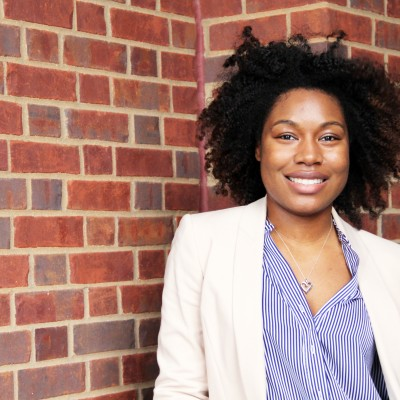
\includegraphics[width=0.5\linewidth]{input/p1-1-1.jpg}
  \caption{Input p1-1-1.jpg, 400x400 pixels}
\end{subfigure}
\begin{subfigure}{0.5\textwidth}
  \centering
  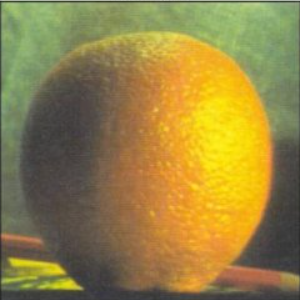
\includegraphics[width=0.5\linewidth]{input/p1-1-2.png}
  \caption{Input p1-1-2.jpg, 300x300 pixels}
\end{subfigure}%
\begin{subfigure}{0.5\textwidth}
  \centering
  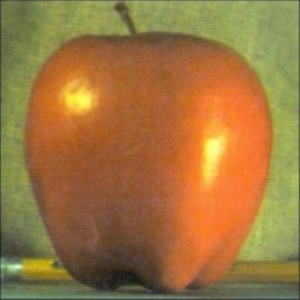
\includegraphics[width=0.5\linewidth]{input/p1-1-3.png}
  \caption{Input p1-1-3.jpg, 300x300 pixels}
\end{subfigure}
 \caption{Images used in experiments}
\label{fig:Input-images}
\end{figure}



\section{Convolution}

The implementation of this function has the following signature:

\begin{lstlisting}[language=python][h!]
convolve(img_input, kernel, padding_type = 'zero', padding_color = 0, normalize = False):
\end{lstlisting}

The kernels tested are shown in figure \ref{fig:conv-kernels}.
 
\begin{figure}[h!]
\centering
\begin{subfigure}{0.3\textwidth}
  \centering
  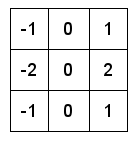
\includegraphics[width=0.5\linewidth]{figs/sobel.png}
  \caption{Sobel}
\end{subfigure}%
\begin{subfigure}{0.3\textwidth}
  \centering
  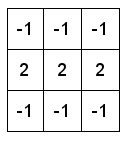
\includegraphics[width=0.5\linewidth]{figs/line.png}
  \caption{Line detector}
\end{subfigure}%
\begin{subfigure}{0.3\textwidth}
  \centering
  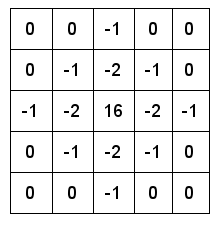
\includegraphics[width=0.5\linewidth]{figs/laplacian-of-gaussian.png}
  \caption{Laplacian of Gaussian}
\end{subfigure}
\begin{subfigure}{0.3\textwidth}
  \centering
  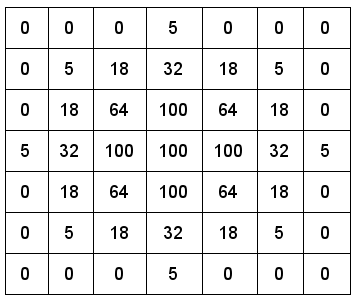
\includegraphics[width=0.9\linewidth]{figs/gaussian.png}
  \caption{Gaussian}
\end{subfigure}%
\begin{subfigure}{0.7\textwidth}
  \centering
  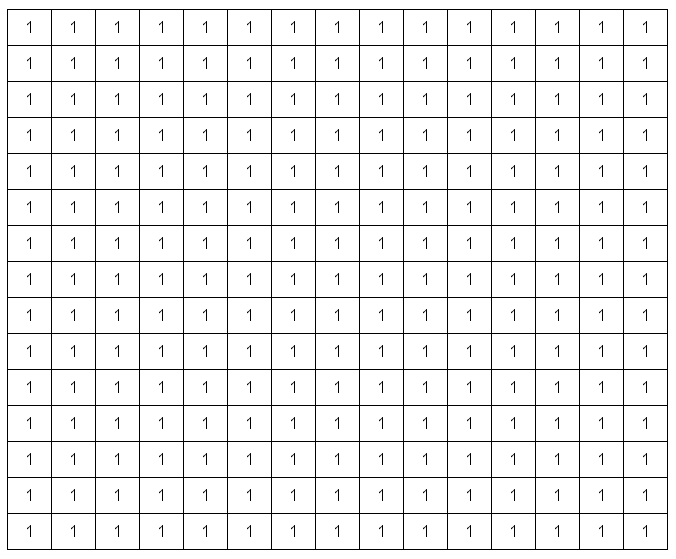
\includegraphics[width=0.9\linewidth]{figs/media.png}
  \caption{Media}
\end{subfigure}
 \caption{Images used in experiments}
\label{fig:conv-kernels}
\end{figure}

Results for each kernel are shown in figure \ref{fig:conv-results}. In the case of the sobel kernel, it corresponds to the vertical component (sobel filter has vertical and horizontal components), thus the results highlights the vertical lines (more clear in the wall of brick). Analyzing the pattern in the line detector it seems like an horizontal line, thus in the result of this kernel, vertical lines disappears. In the case of the Laplacian of Gaussian (LoG) it is working as an edge detector. The media and Gaussian the the result is a blurred images, but in the case of the media kernel the result is bigger because of the size of the kernel.

\begin{figure}[h!]
\centering
\begin{subfigure}{0.3\textwidth}
  \centering
  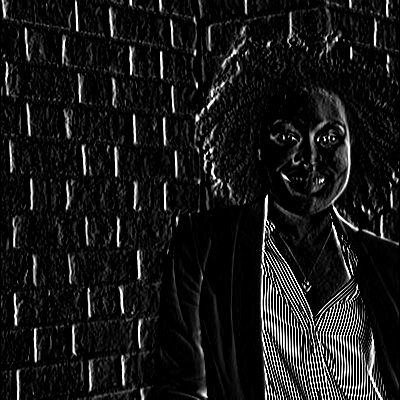
\includegraphics[width=0.9\linewidth]{output/sobel.jpg}
  \caption{Sobel}
\end{subfigure}%
\begin{subfigure}{0.3\textwidth}
  \centering
  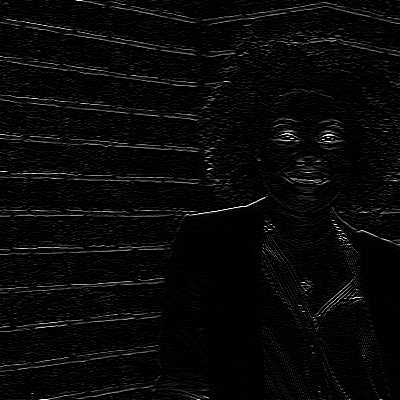
\includegraphics[width=0.9\linewidth]{output/horizontalLine.jpg}
  \caption{Line detector}
\end{subfigure}%
\begin{subfigure}{0.3\textwidth}
  \centering
  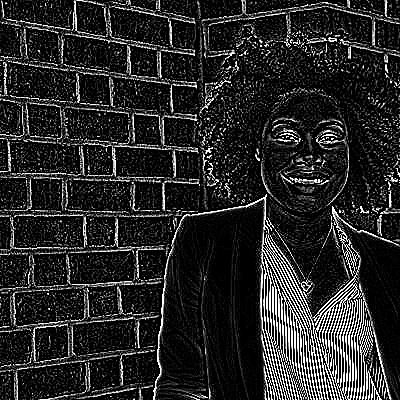
\includegraphics[width=0.9\linewidth]{output/laplasOfGaussi.jpg}
  \caption{Laplacian of Gaussian}
\end{subfigure}
\begin{subfigure}{0.5\textwidth}
  \centering
  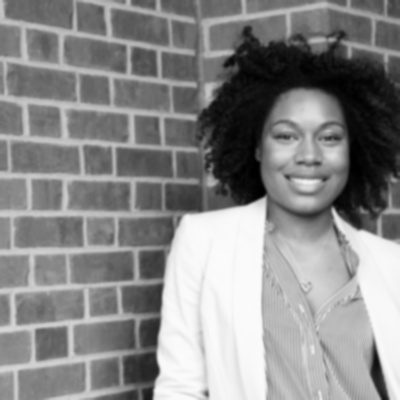
\includegraphics[width=0.5\linewidth]{output/gaussian.jpg}
  \caption{Gaussian}
\end{subfigure}%
\begin{subfigure}{0.5\textwidth}
  \centering
  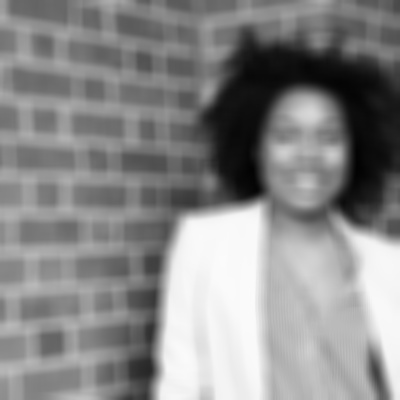
\includegraphics[width=0.5\linewidth]{output/media.jpg}
  \caption{Media}
\end{subfigure}
 \caption{Results of convolution}
\label{fig:conv-results}
\end{figure}

Different kinds of padding are available: $zero, mirror$ and $constant$, the results for different padding strategies are shown in figure \ref{fig:padding-strategy}.

The zero padding suffers of white borders, this may not be logical since 0 is equivalent to black, but if we analyze the convolution kernel (laplacian of gaussian) it makes sense. Mirror padding has the best results because it does not saturate the borders with an specific color, contrary to zero padding, the constant padding with $c=255$ turns the borders with black, the constant padding with $c=128$ has the most similar result to mirror approach.

Because of these results, we consider mirror padding in future experiments.

\begin{figure}[h!]
\centering
\begin{subfigure}{0.25\textwidth}
  \centering
  \frame{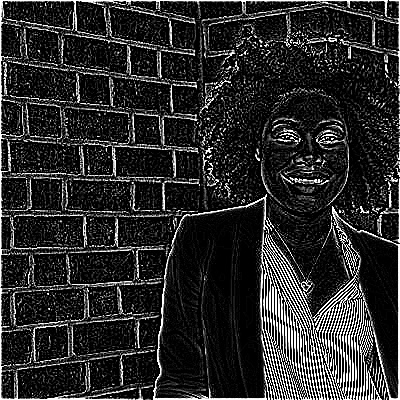
\includegraphics[width=0.9\linewidth]{output/zero.jpg}}
  \caption{Zero padding}
\end{subfigure}%
\begin{subfigure}{0.25\textwidth}
  \centering
  \frame{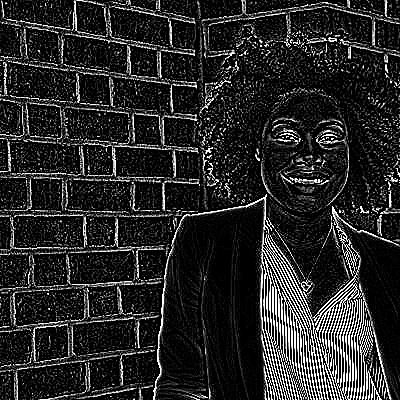
\includegraphics[width=0.9\linewidth]{output/mirror.jpg}}
  \caption{Mirror padding}
\end{subfigure}%
\begin{subfigure}{0.25\textwidth}
  \centering
  \frame{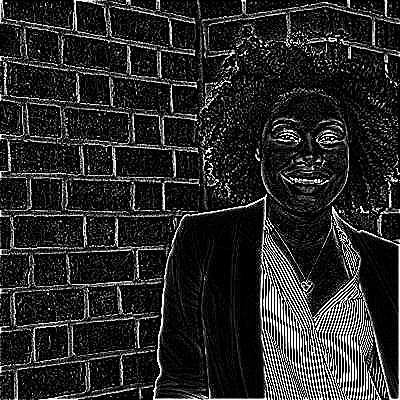
\includegraphics[width=0.9\linewidth]{output/constant128.jpg}}
  \caption{Constant padding $C = 128$}
\end{subfigure}%
\begin{subfigure}{0.25\textwidth}
  \centering
  \frame{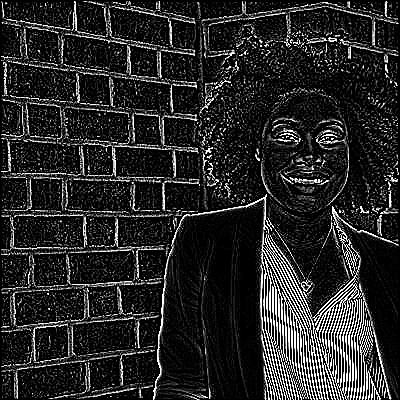
\includegraphics[width=0.9\linewidth]{output/constant255.jpg}}
  \caption{Constant padding $C = 255$}
\end{subfigure}
 \caption{Padding differences}
\label{fig:padding-strategy}
\end{figure}

\vspace{2cm}

The measure of the execution time of the convolution function is shown in table~\ref{tab:time_execution}. Note that since two images are $300 \times 300$ and the other two are $400 \times 400$, we evaluate the time using one of each dimension. In the same way, we consider only one kernel of $ 3 \times 3$ out of the original three.

From the table we can see that the our implementation is much more slower than OpenCV one, this is because the OpenCV library has its methods optimized, an option to improve our implementation is to use $cython$\footnote{\url{http://www.pyimagesearch.com/2017/08/28/fast-optimized-for-pixel-loops-with-opencv-and-python/} shows a solution for this problem.}

\begin{table}[h!]
\centering
\begin{tabular}{|l|l|l|c|r|r|r|}
\hline
\multicolumn{2}{|c|}{\textit{\textbf{Image}}} & \multicolumn{2}{c|}{\textit{\textbf{kernel}}} & \multicolumn{2}{c|}{\textit{\textbf{time execution(seconds)}}} & \multicolumn{1}{c|}{\multirow{2}{*}{\textit{\textbf{Speedup}}}} \\ \cline{1-6}
\multicolumn{1}{|c|}{\textit{\textbf{name}}} & \multicolumn{1}{c|}{\textit{\textbf{dimension}}} & \multicolumn{1}{c|}{\textit{\textbf{name}}} & \textit{\textbf{dimension}} & \multicolumn{1}{c|}{\textit{\textbf{\begin{tabular}[c]{@{}c@{}}Our \\ implementation\end{tabular}}}} & \multicolumn{1}{c|}{\textit{\textbf{OpenCV}}} & \multicolumn{1}{c|}{} \\ \hline
\multirow{4}{*}{p1-1-1.jpg} & \multirow{4}{*}{400x400} & Sobel & 3x3 & 1.0571 & 0.0002 & 5285.5 \\ \cline{3-7} 
 &  & Laplacian of gaussian & 5x5 & 1.1044 & 0.0004 & 2761 \\ \cline{3-7} 
 &  & Gaussian & 7x7 & 1.1191 & 0.0008 & 1398 \\ \cline{3-7} 
 &  & Media & 15x15 & 1.2273 & 0.0026 & 472 \\ \hline
\multirow{4}{*}{p1-1-2.png} & \multirow{4}{*}{300x300} & Sobel & 3x3 & 0.5934 & 0.0001 & 5934 \\ \cline{3-7} 
 &  & Laplacian of gaussian & 5x5 & 0.6023 & 0.0002 & 3011 \\ \cline{3-7} 
 &  & Gaussian & 7x7 & 0.6175 & 0.0004 & 1543 \\ \cline{3-7} 
 &  & Media & 15x15 & 0.7376 & 0.0024 & 307 \\ \hline
\end{tabular}
\caption{Measures of the execution time}
\label{tab:time_execution}
\end{table}


\section{Gaussian Pyramid}

The implementation of the Gaussian pyramid follows the next structure:

\begin{lstlisting}[language=python][h!]
class gaussian_pyramid:
    pyramid = []
    '''
    Initialize the pyramid based on an base image, the number of 
    level and a kernel (Gaussian kernel is the default)
    '''
    def __init__(self, img, levels, kernel = None, gauss_kernel_par= 0.3):
    '''
    interpolates the missing information
    '''
    def interpolation(self,x,y,v, interp = 'bilinear'):
	'''
    upsamples an image, using the desired interpolation method
    '''
    def up_sample(self, image, size, interp = 'bilinear'):
    '''
    downsamples an image, using the desired padding strategy
    '''
    def down_sample(self, image, size, padding_type = 'mirror', 
	'''
    Implements the down operation of the pyramid using the upsample function
    '''
    def down(self, level):
	'''
    Implements the up operation of the pyramid using the downsample function
    '''
    def up(self, level): #downsample the image
    '''
    builts the whole pyramid using up function
    '''
    def build(self):
    '''
    returns the desired level of the pyramid
    '''
    def get(self, level):
    '''
    plots each pyramid level
    '''
    def show(self, name = 'gauss_pyramid'):
\end{lstlisting}

We decided this architecture because it needs to compute each level of the pyramid just once, this is useful when function $get$ is implement recovering each level in $O(1)$, in the same way, this implementation is more transparent for an user, allowing easy and fast use of the pyramid as shown below. 

\begin{lstlisting}[language=python][h!]
pyramid = gaussian_pyramid(img, levels = 7)
pyramid.build()
\end{lstlisting}

Some details of the implementation includes: it can handle multichannel and grayscale images indifferently, it implements only bilinear interpolation\footnote{Based on \url{http://supercomputingblog.com/graphics/coding-bilinear-interpolation/}}, the $down$ function may not return an image of the size of the original one whenever the height or width of the image is odd.

The results of the applying the $up$ function to built the pyramid are shown in figure \ref{fig:gaussian_pyramid}

\begin{figure}[h!]
\centering
  \centering
  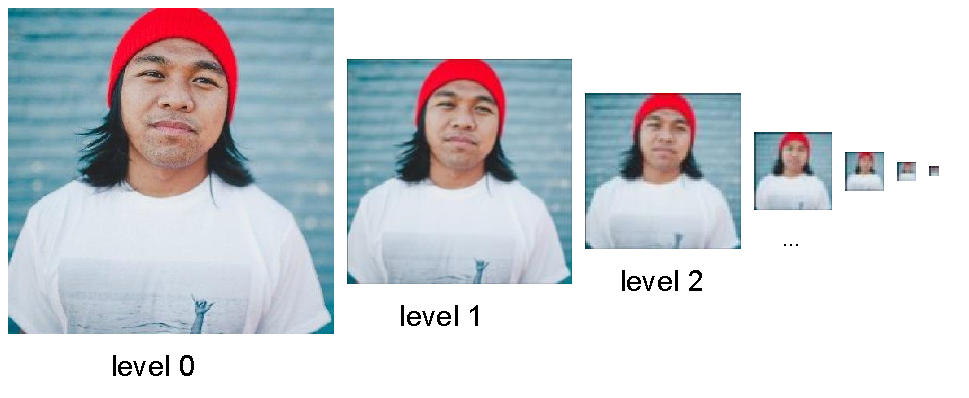
\includegraphics[width=0.9\linewidth]{output/gaussianPyramid.pdf}
  \caption{Gaussian Pyramid}
\label{fig:gaussian_pyramid}
\end{figure}

The result of the $down$ function comparing with the original pyramid level are shown in figure \ref{fig:down-gauss-results}. It can be seen that the upsampled image is not equal to the original one, there is a lost of information that is not recoverable.

\begin{figure}[!h]
\centering
\begin{subfigure}{0.5\textwidth}
  \centering
  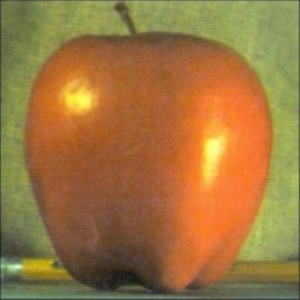
\includegraphics[width=0.8\linewidth]{input/p1-1-3.png}
  \caption{Original image}
\end{subfigure}%
\begin{subfigure}{0.5\textwidth}
  \centering
  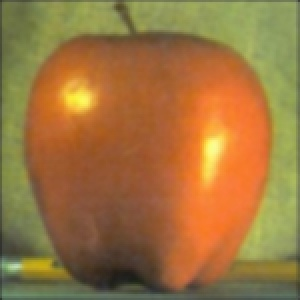
\includegraphics[width=0.8\linewidth]{output/upSample.jpg}
  \caption{Up sampled image}
\end{subfigure}%
 \caption{Comparison of results of $down$ function}
\label{fig:down-gauss-results}
\end{figure}

\section{Laplacian Pyramid}

Similar to Gaussian Pyramid, the implementation of the Laplacian Pyramid, follows the next model:

\begin{lstlisting}[language=python][h!]
class laplacian_pyramid:
    pyramid = []
    '''
    Initialize the pyramid based on the last level of gaussian 
    pyramid,the number of levels and a kernel are of the gaussian
    pyramid
    '''
    def __init__(self, img, levels, kernel = None, gauss_kernel_par = 0.3):  
    '''
    Addition or subtraction an image of level "i" of the gaussian 
    pyramid with the upsampled image of the level i+1 
    '''
    def gauss_operation(self, gauss_cur, gauss_down, operation = '-'):
	'''
    upsamples an image with the down function of the gaussian pyramid
    '''
    def up_sample(self, image, size):
    '''
    upsample an image of a level i of the laplacian pyramid and 
    adds the image of level i+1 of the gaussian pyramid, obtaining 
    the images of the level i of the gaussian pyramid
    '''
    def down(self, up_level_img, cur_level_img):
    '''
    Implements the up operation of the pyramid using the downsample 
    function, this function allows us create one level the 
    laplacian pyramid
    '''
    def up(self, level, gaussian_pyramid):
    '''
    builts the whole pyramid using down function
    '''
    def build(self):  
    '''
    Reconstruct the original image using the laplacian pyramid
    '''
    def reconstruct(self):
    '''
    returns the desired level of the pyramid
    '''
    def get(self, level):
    '''
    plots each pyramid level
    '''
    def show(self, name = 'laplace_pyramid'):
      
\end{lstlisting}

As in the Gaussian implementation, we choose this architecture in order to compute each level of the pyramid just once, this be useful in the blending implementation.

Some details of the implementation includes: it can handle multichannel and grayscale images indifferently, the function  $gauss_operation$ can handle the cases where the upsampled image does not have the same shape as the current level, the $down$ function up samples an image and sum it with another image, this function is the core the the $reconstruct$ function. The last level is equal in the Laplacian pyramid   and Gaussian pyramid.

The logic to reconstruct the image is shown in figure \ref{fig:reconstruction-laplace}, initially, the last level $i$ of the Laplacian pyramid is upsampled, and then is added to the level $i-1$, the first row of figure \ref{fig:reconstruction-laplace} shows the elements inside the Laplacian pyramid, the second row shows the intermediate results of upsampling an image that was previously added with the corresponding Laplace pyramid level. Note that the results of the sum up (third row in figure \ref{fig:reconstruction-laplace}) are more clean an look like the original image.

\begin{figure}[h!]
\hspace{-1cm}
  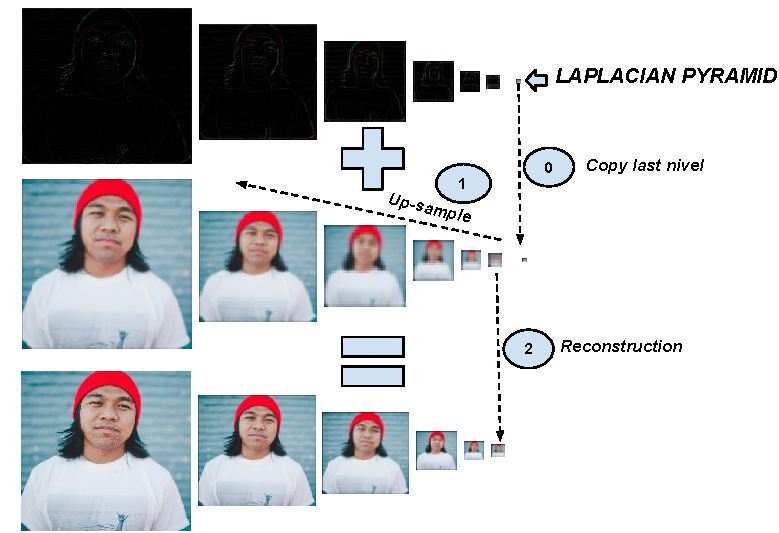
\includegraphics[width=1.1\linewidth]{output/reconstructionImage.pdf}
  \caption{Reconstruction process}
\label{fig:reconstruction-laplace}
\end{figure}

\section{Blending}

The function $blending$ receives two images, the mask and the pyramid levels, it returns the blended image.

\begin{lstlisting}[language=python][h!]
blending(img_a, img_b, mask, level = 2)
\end{lstlisting}

Initially, the Laplacian pyramid of $image_a, image_b$ and Gaussian Pyramid of the $mask$ are build.

\begin{lstlisting}[language=python][h!]
lp_a = lp.laplacian_pyramid(img_a,level)
lp_b = lp.laplacian_pyramid(img_b,level)
gp_mask = gp.gaussian_pyramid(mask,level)
lp_a.build()
lp_b.build()
gp_mask.build()
\end{lstlisting}

Next, the images of each level of Laplacian pyramids are joint using its corresponding level in Gaussian pyramid of the $mask$, they are stored in $mid$.

\begin{lstlisting}[language=python][h!]
mid = []
for i in range(level - 1, -1, -1):
    mask = gp_mask.get(i)
    joint = combine(lp_a.get(i), lp_b.get(i), mask)
    mid.append(joint)
\end{lstlisting}

Finally, the same process of reconstruction as in Laplacian pyramid is done, this  yields in the blended image. As explained in the previous section, the function $down$ of the Laplacian pyramid will upsample \textit{img\_blend}(the first time \textit{img\_blend} is equivalent to the union of the last levels of Gaussian pyramids) and will sum it up with $mid[i]$, this operation is the inverse of the $up$ operation used to build the Laplacian pyramid.

\begin{lstlisting}[language=python][h!]
img_blend = mid[0]
for i in range(1, len(mid)):
	img_blend = lp_a.down(img_blend, mid[i])
return img_blend
\end{lstlisting}

The main problem during implementation was related with the size of the up sampled image and the current level: when the width or height was odd, we "lose" a row or a columns. Another problem was related with multichannel images, it is better to have a function that blends RGB or grayscale images without extra parameters or more complicated stuff, in a transparent way to the user. Thus, our implementation overcomes these problems and has not limitation in this sense, moreover there is a previous step that checks whether the size of the input images are equal such that it resize them to get valid shapes. Note that the implementation allows to set the $mask$ with left-right blending, bottom-up blending and also load a binary image as $mask$.

We performed extensive experiments with different images. The results of the blending are shown in the sub figures~\ref{fig:blending-b}, ~\ref{fig:blending-c} and ~\ref{fig:blending-d}. The blending generated by the OpenCV algorithm is shown in the sub figure~\ref{fig:blending-a}. The result of our implementation is very similar to the OpenCV one, therefore, we conclude that our implementation is going well.

\begin{figure}[h!]
\centering
\begin{subfigure}{0.33\textwidth}
  \centering
  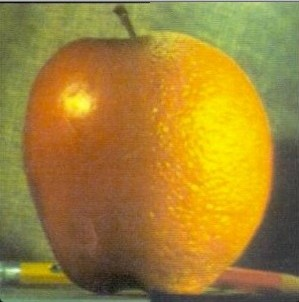
\includegraphics[width=0.8\linewidth]{output/blendedOpenCV.jpg}
  \caption{blending with \href{http://docs.opencv.org/3.1.0/dc/dff/tutorial_py_pyramids.html}{\textit{OpenCV}}.}
  \label{fig:blending-a}
\end{subfigure}%
\begin{subfigure}{0.33\textwidth}
  \centering
  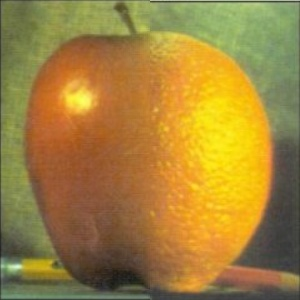
\includegraphics[width=0.8\linewidth]{output/blending1.jpg}
  \caption{Left-right blending}
  \label{fig:blending-b}
\end{subfigure}%
\begin{subfigure}{0.33\textwidth}
  \centering
  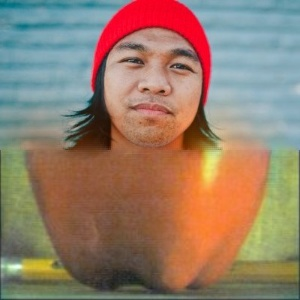
\includegraphics[width=0.8\linewidth]{output/blending2.jpg}
  \caption{Bottom-up blending}
  \label{fig:blending-c}
\end{subfigure}
\begin{subfigure}{0.7\textwidth}
  \centering
  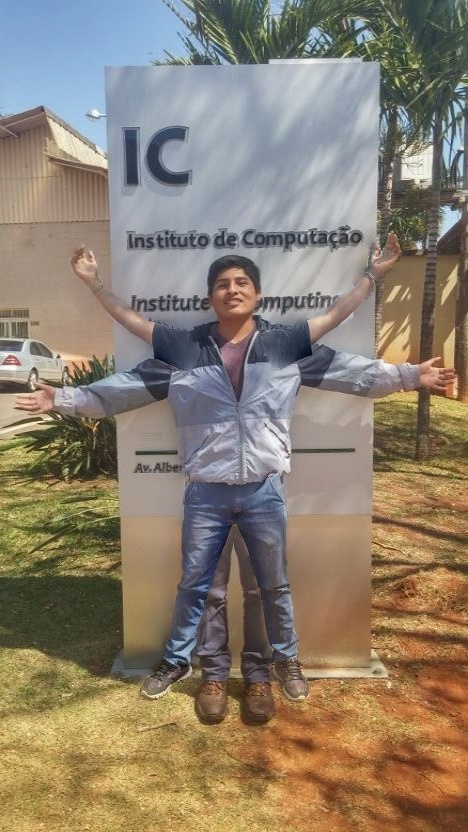
\includegraphics[width=0.8\linewidth]{output/blending.jpg}
  \caption{Binary image blending}
  \label{fig:blending-d}
\end{subfigure}%
 \caption{Blending results}
\label{fig:blending}

\end{figure}





\section{Exploring Fourier Space}

The results for the phase and magnitude extraction are shown in figures \ref{fig:low-magnitude}, \ref{fig:high-magnitude}, \ref{fig:high-phase} and \ref{fig:low-phase}

\begin{figure}[h!]
\centering
\begin{subfigure}{0.2\textwidth}
  \centering
  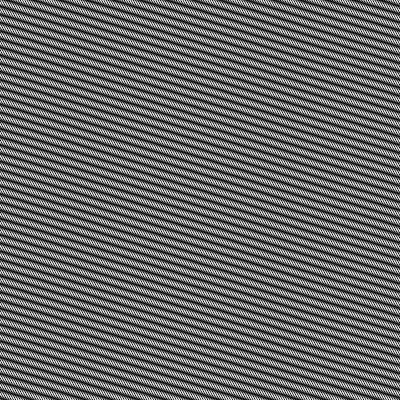
\includegraphics[width=0.95\linewidth]{output/magnitud_low_1.jpg}
  \caption{1st lowest}
\end{subfigure}%
\begin{subfigure}{0.2\textwidth}
  \centering
  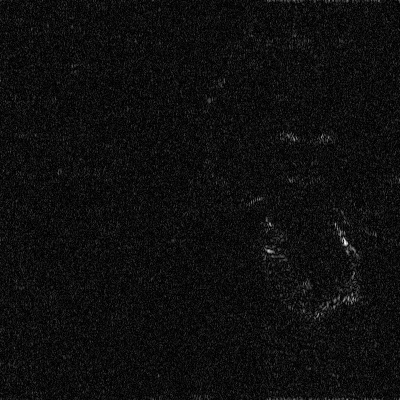
\includegraphics[width=0.95\linewidth]{output/magnitud_low_25.jpg}
  \caption{25 \% lowest}
\end{subfigure}%
\begin{subfigure}{0.2\textwidth}
  \centering
  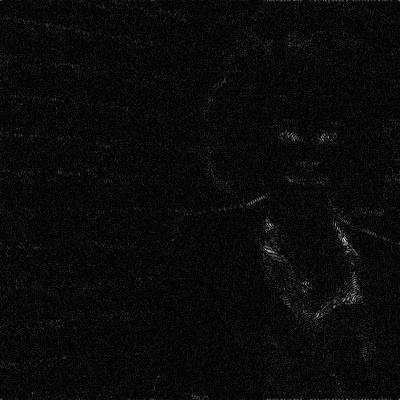
\includegraphics[width=0.95\linewidth]{output/magnitud_low_50.jpg}
  \caption{50 \% lowest}
\end{subfigure}%
\begin{subfigure}{0.2\textwidth}
  \centering
  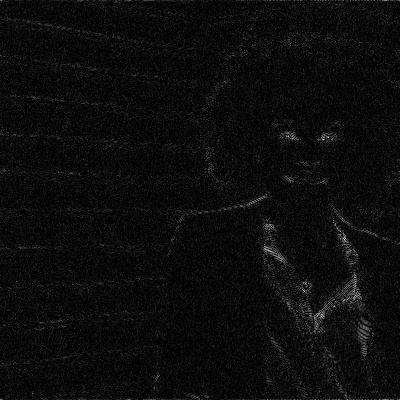
\includegraphics[width=0.95\linewidth]{output/magnitud_low_75.jpg}
  \caption{75 \% lowest}
\end{subfigure}%
\begin{subfigure}{0.2\textwidth}
  \centering
  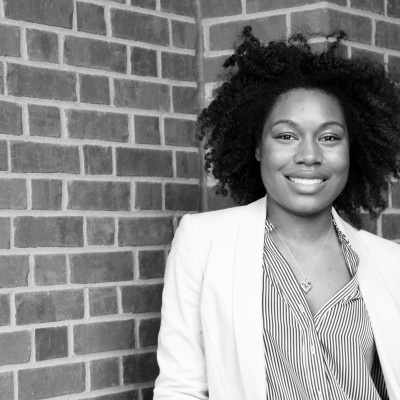
\includegraphics[width=0.95\linewidth]{output/magnitud_low_100.jpg}
  \caption{100 \% lowest}
\end{subfigure}%
 \caption{Low magnitude extraction}
\label{fig:low-magnitude}
\end{figure}

Getting the lowest values of the magnitude yields in images that shows groups of points that represents the woman of the original image. Note that the first image (the 1st lowest) seems to not have relation with original one.

\begin{figure}[h!]
\centering
\begin{subfigure}{0.2\textwidth}
  \centering
  
\includegraphics[width=0.95\linewidth]{output/magnitud_high_1}
  \caption{1st highest}
\end{subfigure}%
\begin{subfigure}{0.2\textwidth}
  \centering
  
\includegraphics[width=0.95\linewidth]{output/magnitud_high_25}
  \caption{25 \% highest}
\end{subfigure}%
\begin{subfigure}{0.2\textwidth}
  \centering
  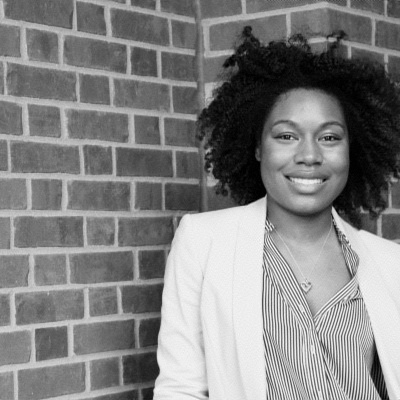
\includegraphics[width=0.95\linewidth]{output/magnitud_high_50}
  \caption{50 \% highest}
\end{subfigure}%
\begin{subfigure}{0.2\textwidth}
  \centering
  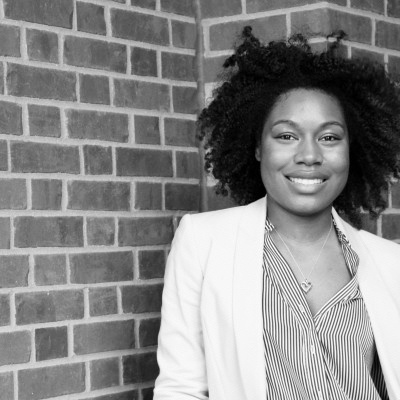
\includegraphics[width=0.95\linewidth]{output/magnitud_high_75}
  \caption{75 \% highest}
\end{subfigure}%
\begin{subfigure}{0.2\textwidth}
  \centering
  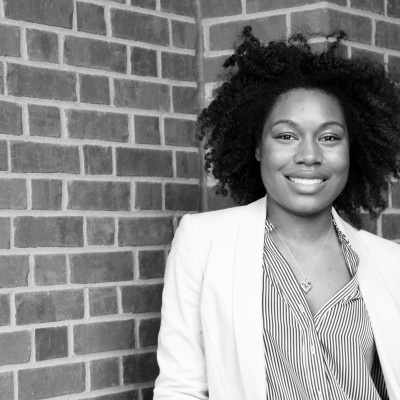
\includegraphics[width=0.95\linewidth]{output/magnitud_high_100}
  \caption{100 \% highest}
\end{subfigure}%
 \caption{High magnitude extraction}
\label{fig:high-magnitude}
\end{figure}

We can see in the figure \ref{fig:high-magnitude}, the the effect of taking the 1st greatest value creates an image that seems to not have relation with the original one, but, in the rest of images the difference is really small, it is just a little more clear while taking higher values.

\begin{figure}[h!]
\centering
\begin{subfigure}{0.2\textwidth}
  \centering
  
\includegraphics[width=0.95\linewidth]{output/phase_low_1.jpg}
  \caption{1st lowest}
\end{subfigure}%
\begin{subfigure}{0.2\textwidth}
  \centering
  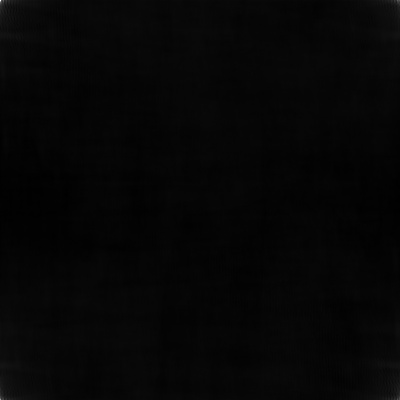
\includegraphics[width=0.95\linewidth]{output/phase_low_25.jpg}
  \caption{25 \% lowest}
\end{subfigure}%
\begin{subfigure}{0.2\textwidth}
  \centering
  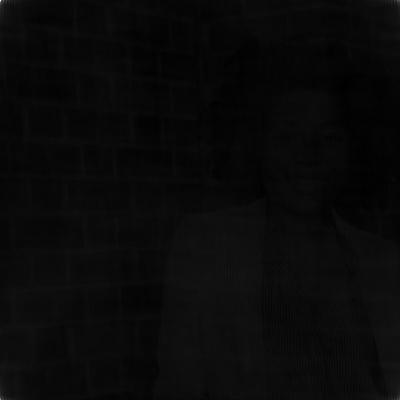
\includegraphics[width=0.95\linewidth]{output/phase_low_50.jpg}
  \caption{50 \% lowest}
\end{subfigure}%
\begin{subfigure}{0.2\textwidth}
  \centering
  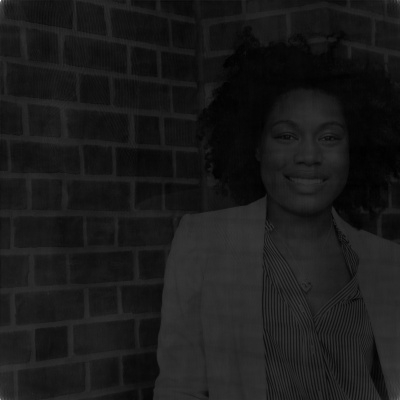
\includegraphics[width=0.95\linewidth]{output/phase_low_75.jpg}
  \caption{75 \% lowest}
\end{subfigure}%
\begin{subfigure}{0.2\textwidth}
  \centering
  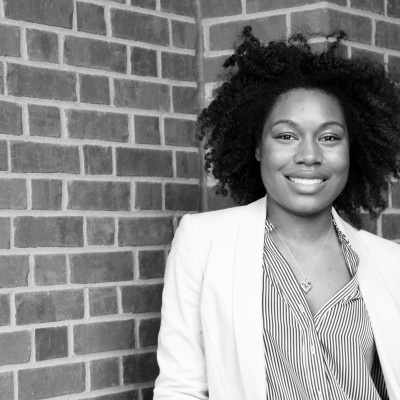
\includegraphics[width=0.95\linewidth]{output/phase_low_100.jpg}
  \caption{100 \% lowest}
\end{subfigure}%
 \caption{Low phase extraction}
\label{fig:low-phase}
\end{figure}

Also, we can see in the figure~\ref{fig:low-phase} that while we take less quantity of lower values, the intensity of the image is less. This occurs because the phase carries a large part of the spatial information of the image, therefore, while we take more values, then major features of the image are preserved.


\begin{figure}[h!]
\centering
\begin{subfigure}{0.2\textwidth}
  \centering
  
\includegraphics[width=0.95\linewidth]{output/phase_high_1.jpg}
  \caption{1st highest}
\end{subfigure}%
\begin{subfigure}{0.2\textwidth}
  \centering
  
\includegraphics[width=0.95\linewidth]{output/phase_high_25.jpg}
  \caption{25 \% highest}
\end{subfigure}%
\begin{subfigure}{0.2\textwidth}
  \centering
  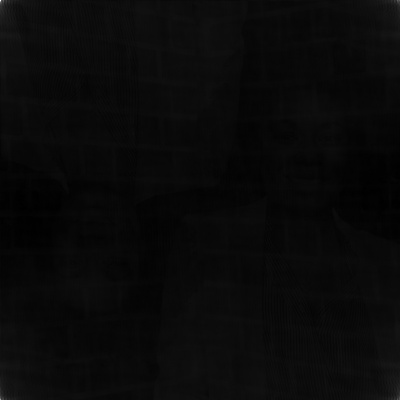
\includegraphics[width=0.95\linewidth]{output/phase_high_50.jpg}
  \caption{50 \% highest}
  \label{fig:high-phase-c}
\end{subfigure}%
\begin{subfigure}{0.2\textwidth}
  \centering
  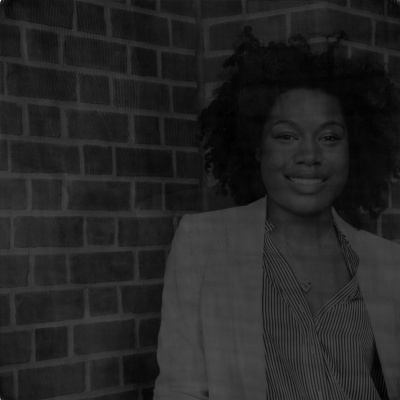
\includegraphics[width=0.95\linewidth]{output/phase_high_75.jpg}
  \caption{75 \% highest}
\end{subfigure}%
\begin{subfigure}{0.2\textwidth}
  \centering
  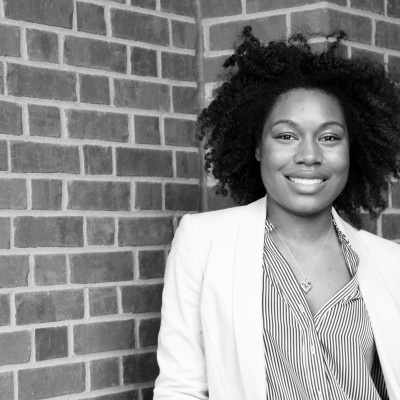
\includegraphics[width=0.95\linewidth]{output/phase_high_100.jpg}
  \caption{100 \% highest}
\end{subfigure}%
 \caption{High phase extraction}
\label{fig:high-phase}
\end{figure}
Similar to above, in the figure~\ref{fig:high-phase} we can see that the intensity of the image is less while we taking less quantity of high values. Also we can see that in the sub figure~\ref{fig:high-phase-c} the image suffer a modification, creating a woman of inverted shape next to the original woman. This occurs because we take only high values altering the original feature and the intensity of the image, modifying the original woman.

Comparing results from images \ref{fig:low-magnitude} and \ref{fig:low-phase}, we can see that the changes in phase have a bigger effect (e.g. we lose a lot of information), moreover, comparing \ref{fig:high-magnitude} and \ref{fig:high-phase}, the results of getting the highest values in the magnitude seems to not have any effect, on the other hand, getting the 75 \% of the highest phase values yields in a big change. Thus the phase is more important than the magnitude.


\section{Frequency Blending}

In order to blend the images using the frequency domain, we convert the masked image to the frequency domain and focus on approaches to combine these frequency domains images. We consider 6 ideas of combination. 

\begin{itemize}
\item The first one is named "left-right", this method takes a left half of the first frequency domain image and the right half of the another. The results of this method are shown in figure \ref{fig:left-right}. These images shows a successful combination of the original images but the intersection point is not as smooth as it would be expected, this is because in the frequency domain it is not possible to smooth just a small part of the image (e.g. intersection points), the alternative of blurring (e.g. taking out low frequencies) before applying the left-right blend would end up in the same result but blurred in the whole image and not just the intersection points.

\begin{figure}[h!]
\centering
\begin{subfigure}{0.4\textwidth}
  \centering
  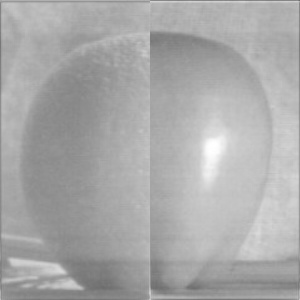
\includegraphics[width=0.7\linewidth]{output/left_right1.jpg}
  \caption{Left-right blending apple-orange}
\end{subfigure}%
\begin{subfigure}{0.4\textwidth}
  \centering
  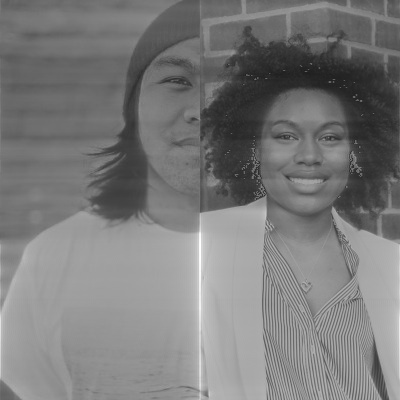
\includegraphics[width=0.7\linewidth]{output/left_right2.jpg}
  \caption{Left-right blending woman-man}
\end{subfigure}%
\caption{Left-right blending}
\label{fig:left-right}
\end{figure}

\item The second method is named "bottom-up", this is similar to the "left\_right" approach but takes the up half of one image and the bottom half of the another. The results of this method are shown in figure \ref{fig:bottom_up}. As equal to the previous approach, the images were successfully joined but with a sharp change in the intersection. Different from previous approach, some vertical shadows appear (left-right approach has horizontal shadows), this highlights the intersection change.

\begin{figure}[h!]
\centering
\begin{subfigure}{0.4\textwidth}
  \centering
  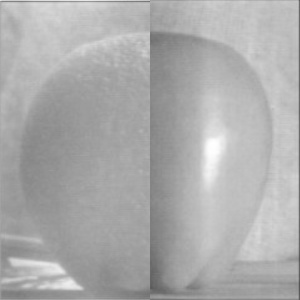
\includegraphics[width=0.7\linewidth]{output/bottom_up1.jpg}
  \caption{Bottom-up blending apple-orange}
\end{subfigure}%
\begin{subfigure}{0.4\textwidth}
  \centering
  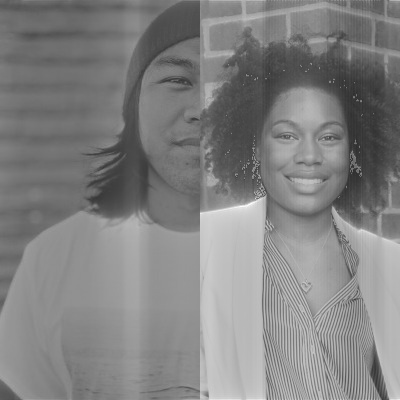
\includegraphics[width=0.7\linewidth]{output/bottom_up2.jpg}
  \caption{Bottom-up blending woman-man}
\end{subfigure}%
\caption{Bottom-up blending}
\label{fig:bottom_up}
\end{figure}

\item The third method is named "centered", this takes the lowest frequencies from one image and the highest frequencies from the other. The results of this method are shown in figure \ref{fig:centered}. Different from previous methods, this approach can not joint the images correctly, it generates a strange combination, this happens because we are taking the lowest frequencies of the second image. Note that in the second combination, the low frequency part is more visible, this due to the quantities of low frequencies that woman image contains.

\begin{figure}[h!]
\centering
\begin{subfigure}{0.4\textwidth}
  \centering
  \includegraphics[width=0.7\linewidth]{output/centered1.jpg}
  \caption{Centered blending apple-orange}
\end{subfigure}%
\begin{subfigure}{0.4\textwidth}
  \centering
  \includegraphics[width=0.7\linewidth]{output/centered2.jpg}
  \caption{Centered blending woman-man}
\end{subfigure}%
\caption{Centered blending}
\label{fig:centered}
\end{figure}

\item The fourth method is named 'chessboard', it combines the frequency images taking one pixel from one image and the next from the other, this creates a kind of chessboard of the frequency images. The results of this method are shown in figure \ref{fig:chessboard}. Due the extreme combination of frequency images, the characteristics of the images mix up generating shadows and photographic negatives.

\begin{figure}[h!]
\centering
\begin{subfigure}{0.4\textwidth}
  \centering
  \includegraphics[width=0.7\linewidth]{output/chessboard1.jpg}
  \caption{Chessboard blending apple-orange}
\end{subfigure}%
\begin{subfigure}{0.4\textwidth}
  \centering
  \includegraphics[width=0.7\linewidth]{output/chessboard2.jpg}
  \caption{Chessboard blending woman-man}
\end{subfigure}%
\caption{Chessboard blending}
\label{fig:chessboard}
\end{figure}

\item The fifth method is named "sliding-rows", this creates horizontal stripes intercalating values from the both frequency images. The results of this method are shown in figure \ref{fig:sliding-rows}. These results are interesting because the same method gives really different results, in the case of the apple-orange blending the left side of the image look like a kind of texture of the image (something like a local binary pattern), and the woman-man blending is much more better, the explanation for this effect may be related with the properties of the images, as equal as is centered blending.

\begin{figure}[h!]
\centering
\begin{subfigure}{0.4\textwidth}
  \centering
  \includegraphics[width=0.7\linewidth]{output/sliding_rows1.jpg}
  \caption{Sliding-rows blending apple-orange}
\end{subfigure}%
\begin{subfigure}{0.4\textwidth}
  \centering
  \includegraphics[width=0.7\linewidth]{output/sliding_rows2.jpg}
  \caption{Sliding-rows blending woman-man}
\end{subfigure}%
\caption{Sliding-rows blending}
\label{fig:sliding-rows}
\end{figure}

\item The sixth method is named "sliding-columns", this creates vertical stripes intercalating values from the both frequency images. The results of this method are shown in figure~\ref{fig:sliding-columns}. The experiments looks similar to the previous approach but in this case the images are a little bit more lighter.

\begin{figure}[h!]
\centering
\begin{subfigure}{0.4\textwidth}
  \centering
  \includegraphics[width=0.7\linewidth]{output/sliding_columns1.jpg}
  \caption{Sliding-columns blending apple-orange}
\end{subfigure}%
\begin{subfigure}{0.4\textwidth}
  \centering
  \includegraphics[width=0.7\linewidth]{output/sliding_columns2.jpg}
  \caption{Sliding-columns blending woman-man}
\end{subfigure}%
\caption{Sliding-columns blending}
\label{fig:sliding-columns}
\end{figure}

\end{itemize}

Comparing this results with the obtained in the space domain (figure~\ref{fig:comparison-blending}) we can see that the change in the space domain is smoother, this is because the blending in the frequency domain is not fully development. Note that the frequency domain blending only considers grayscale image as inputs.

\begin{figure}[h!]
\centering
\begin{subfigure}{0.5\textwidth}
  \centering
  \includegraphics[width=0.9\linewidth]{output/blending1.jpg}
  \caption{Space domain blending}
\end{subfigure}%
\begin{subfigure}{0.5\textwidth}
  \centering
  \includegraphics[width=0.9\linewidth]{output/left_right1.jpg}
  \caption{Frequency domain blending}
\end{subfigure}%
\caption{Blending comparison}
\label{fig:comparison-blending}
\end{figure}



\end{document}
